\section{Turbulence V}
Since the last problem set is quite long and close to the end of the quarter, the remaining lectures will be sketching out the problems, and you will have the task of filling out the steps.

\subsection{Review}
Let us write the starting point of all of our travels/joy:
\begin{equation}\label{eq:NSwithoddviscos}
    \p_t \v{v} + \v{v} \cdot \nabla \v{v} = -\frac{1}{\rho_0}\nabla p + \nu \nabla^2\v{v} + \nu_0\zhat \times \nabla^2\v{v}
\end{equation}
in the homework you actually take this one step further and consider two odd viscosities. In 2D, we can impose isotropy; we can make the particles spin in the plane, with rotation axis perpendicular to the plane. In 3D, the rotation axis must live in the space, so we can have the possibility of more terms. This is all to say - the model we have been studying in lecture we have taken the liberty of simplifying a little bit, in the interest of not writing down an excessive amount of terms (even though in real materials we of course have a lot of terms - but the statistical mechanical features of many realistic models are captured with simpler models, e.g. modelling magnets via the Ising model).

The last term in Eq. \eqref{eq:NSwithoddviscos} corresponds to the odd viscosity term. We could also consider instead a term $\Omega\zhat \times \v{v}$ corresponding to a Coriolis/body force - odd viscosity is like considering a $k$-dependent Coriolis force of $\Omega \sim \nu^0 k^2$.

We looked at the Taylor-Proudman argument, where we balanced the pressure term and the chiral term, and found that:
\begin{equation}
    \p_z \v{v} \approx 0
\end{equation}
i.e. the chiral term seems to make the 3D system quasi-2D. We saw this in simulations as well, where the vortices in the fluid aligned along the rotation axis.

We also thought about the energy spectrum - for small $k$ we have the Kolmogorov direct cascade, and for large $k$, large $\frac{\nu^0}{\nu} \gg 1$ (and of course $\text{Re} \gg 1$ throughout) we have quasi-2-dimensionalization and get an inverse energy cascade.

\begin{center}
    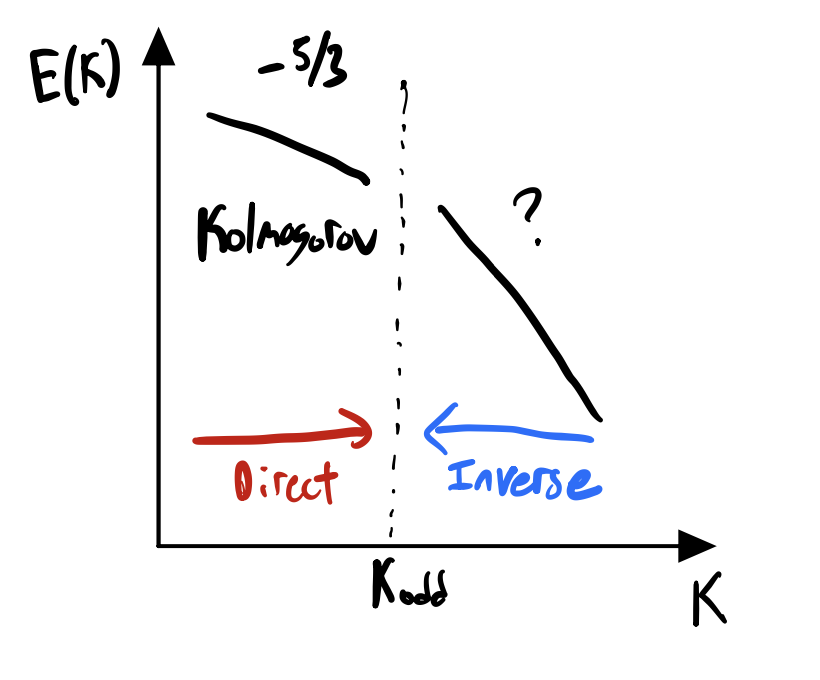
\includegraphics[scale=0.4]{Lectures/Images/lec15-oddpowerspectrum.png}
\end{center}

Note that we still do not know how to connect the two asymptotic regimes in the transition regime of $k = k_{\text{odd}}$. The flow of energy is towards this intermediate scale, where we see pattern formation. Observing that zero $\nu^0$ results in $k_{\text{odd}} = \infty$, we can postulate $k_{\text{odd}} \sim (\nu^0)^{-\alpha}$. 

So our tasks for today - find the power spectrum power law dependence of high $k$ region, then deduce $k_{\text{odd}}$, and then explore the behaviour near this $k_{\text{odd}}$.

We also deduced the Kraichnan formula:
\begin{equation}
    \e \sim \tau(k) k^4E(k)^2
\end{equation}
assuming that the cascade is local in $k$-space, that energy is conserved away from the energy injection, and that $\e$ is linear in $\tau(k)$ (this last assumption is the trickiest assumption to justify/come to grips with). The power spectrum is:
\begin{equation}
    \boxed{E(k) = \left[\frac{\e}{\tau(k)}\right]^{1/2}k^{-2}}
\end{equation}

\subsection{Finishing the Power Spectrum derivation}
Let's review the Kolmogorov analysis. The eddy turnover time is given as:
\begin{equation}
    \tau_{\text{eddy}} \sim \frac{l_k}{v_k} \sim e^{-1/3}k^{-2/3}
\end{equation}
Thus the power spectrum is given by:
\begin{equation}
    E(k) = \left[\frac{\e}{\tau(k)}\right]^{1/2}k^{-2} \sim \left[\frac{\e}{\e^{-1/3}}\right]^{1/2}\left[k^{2/3}\right]^{1/2}k^{-2} = \boxed{\e^{2/3}k^{-5/3}}
\end{equation}
But now what we want to do is the following. We need a hypothesis about what is happening in the inverse cascade region. We recall:
\begin{equation}
    D_t \v{v} = -\frac{1}{\rho_0}\nabla p + \m{\nu & \nu^0 & 0 \\ -\nu^0 & \nu & 0 \\ 0 & 0 & \nu}\Delta\v{v}
\end{equation}
and how the $\nu^0$ symplectic structure allowed the system to support waves/oscillations.

Thus in addition to eddy dynamics, we have wavelike dynamics. Like we have $\tau_k \sim \frac{l_k}{v_k}$ to be the timescale of the eddys, we also have timescale of waves - the period/frequency of a wave. In your homework, you will prove that in the special limit where there is only one odd viscosity, we have:
\begin{equation}
    \omega \sim \nu^0\abs{\v{k}}k_z \sim \nu^0 k^2
\end{equation}
Hence:
\begin{equation}
    \tau_{\text{wave}} \sim \frac{1}{\omega} \sim k^{-2}
\end{equation}
The regimes where one timescale is much shorter than the other are much more comparatively simple to analyze. The regime where they crossover ($\tau_{\text{wave}} \sim \tau_{\text{eddy}}$) is harder to analyze, and tells us about $k_{\text{odd}}$, because both the wave/eddy timescales depend on $k$. Namely:
\begin{equation}
    \nu^0 k_{\text{odd}}^2 = \e^{1/3}k_{\text{odd}}^{2/3} \implies \boxed{k_{\text{odd}} \sim (\nu^0)^{-3/4}}
\end{equation}
If this is true, there is a regime where $k > k_{\text{odd}}$, then the dominant timescale is that of the waves. If we go the Kraichnan formula and plug in the wave timescale, we get:
\begin{equation}
    \boxed{E(k) \sim \left[\e \nu^0 k^2\right]^{1/2}k^{-2} \sim \e^{1/2}(\nu^0)^{1/2}k^{-1}}
\end{equation}
Note that this $E(k)$ has a different $k$ scaling from the Kolmogorov $k^{-5/3}$ and has a dependence on $\nu^0$, arising from the fact that the odd viscosity creates the waves in the fluid.

Let's consider a plot of the spectrum ratio $E(k)/E_0(k)$:

\begin{center}
    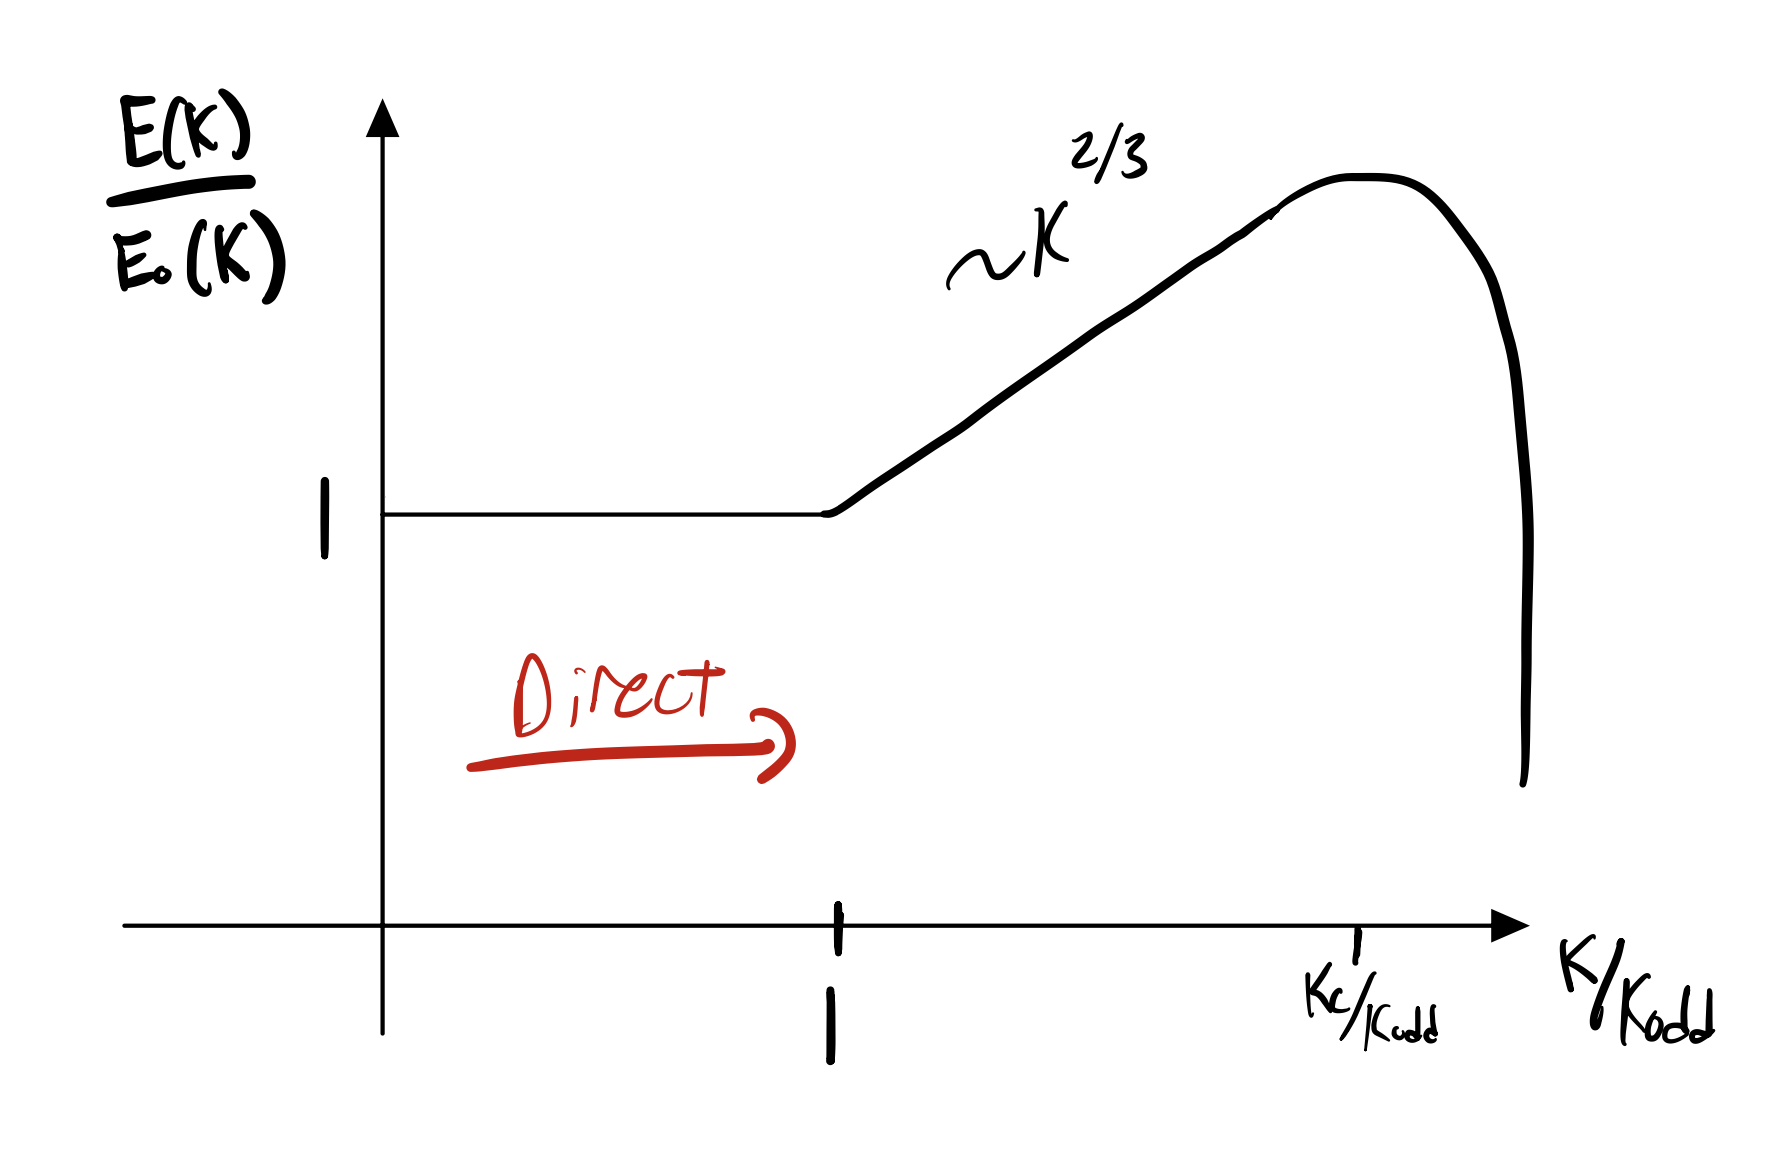
\includegraphics[scale=0.35]{Lectures/Images/lec16-sketch.png}
\end{center}

Where we note that at $k_c$ we have the onset of the dissipative scale. We can estimate this - before, let's look at simulations of a normal fluid $\frac{\nu^0}{\nu} = 0$ and an odd fluid $\frac{\nu^0}{\nu} \gg 1$. In the normal fluid case we see a random distribution of eddys, in the odd viscosity case we see eddy formation on a lengthscale $\sim \frac{1}{k_c}$. We can look at the energy spectrum of such simulations, and we find the structure of Kolmogorov for $k < k_{\text{odd}}$, rising of the power spectrum for $k_{\text{odd}} \leq k \leq k_c$, and the steep dropdown for $k > k_c$.

\begin{center}
    \includegraphics[scale=0.3]{Lectures/Images/lec16-fluidsims.png}
\end{center}


Let us rescale the power spectrum plot above by $k_{\text{odd}}$.

\begin{center}
    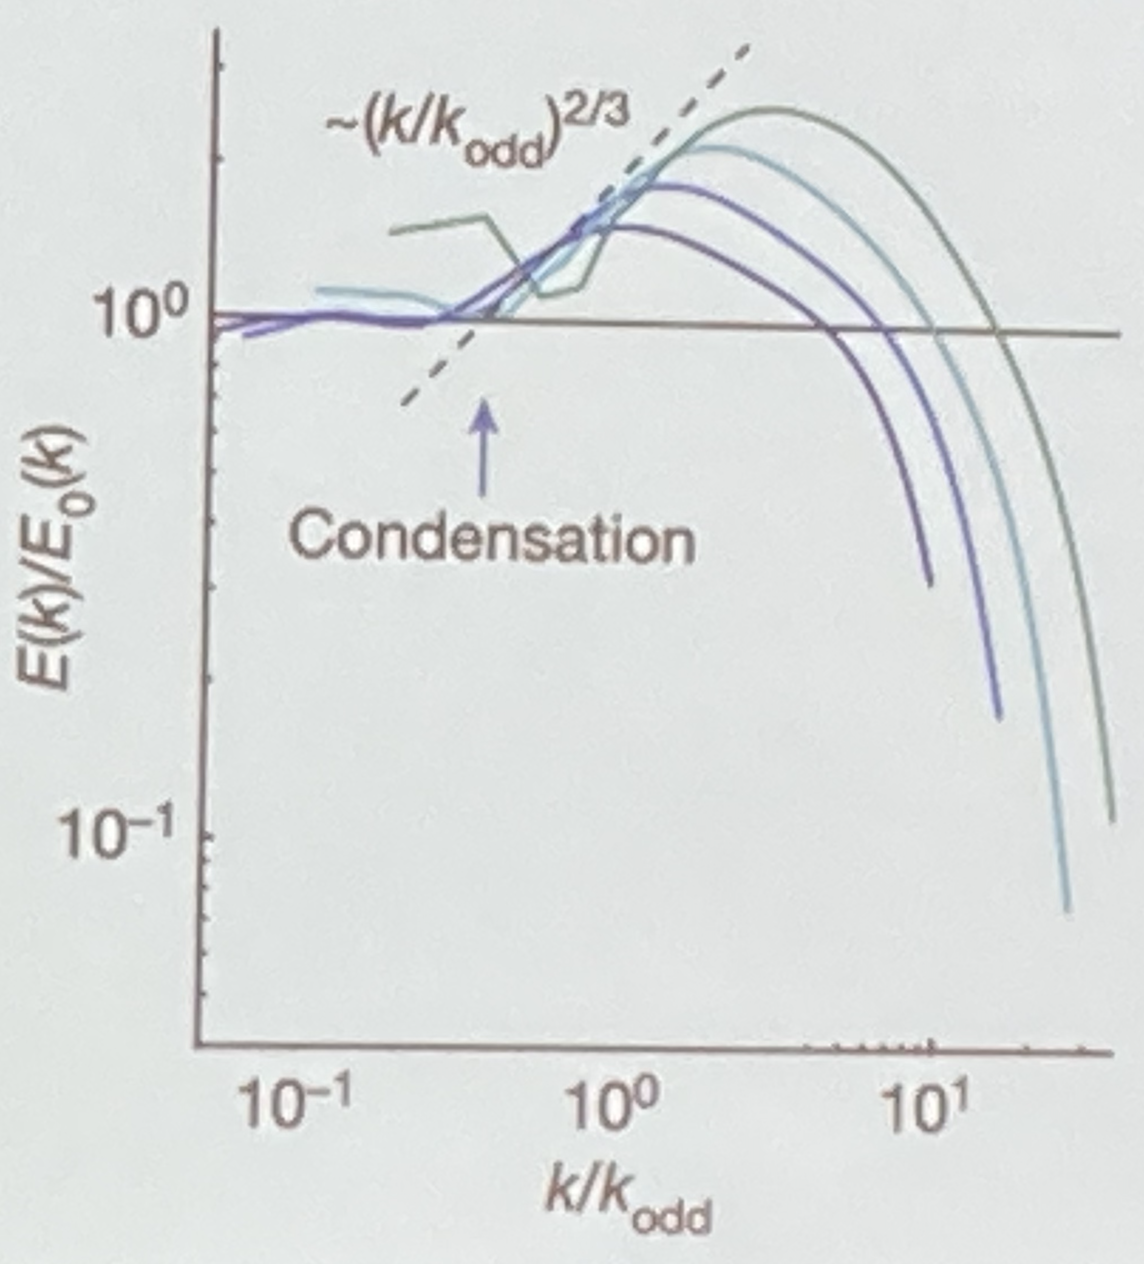
\includegraphics[scale=0.3]{Lectures/Images/lec16-Escaling.png}
\end{center}

We see the curves collapse on one another in the Kolmogorov regime a,d in the $\sim(k/k_{\text{odd}})^{2/3}$ regime, but the maximum shifts, telling us that $k_c$ has some dependence on $\nu^0$ that is different from $k_{\text{odd}}$. Let's see if we can deduce this now. The rate of energy dissipation is given by (coming from $\nu(\nabla \v{v})^2$):
\begin{equation}
    \e_{\text{dis}} \sim \int_{k_{\text{odd}}}^{k_c} \nu k^2 E(k)dk
\end{equation}
Let us carry out this integral:
\begin{equation}
    \e \sim \int_{k_{\text{odd}}}^{k_c}k^2 \e^{1/2}(\nu^0)^{1/2}k^{-1}dk \sim \nu (\nu^0)^{1/2}\e^{1/2}\left.k^2\right|^{k_c}_{k_{\text{odd}}}
\end{equation}
Assuming that $k_c \gg k_{\text{odd}}$ then:
\begin{equation}
    \e \sim \nu (\nu^0)^{1/2}\e^{1/2}k_c^2
\end{equation}
Hence:
\begin{equation}
    \boxed{k_c \sim (\nu^0)^{-1/4}}
\end{equation}
so, if i keep track the initial data of all the maxima of $E(k)/E_0(k)$, we can then plot $k_c$ as a function of $\nu_0/\nu$, and we have evidence for power law scaling of $(\nu^0)^{-1/4}$.

\begin{center}
    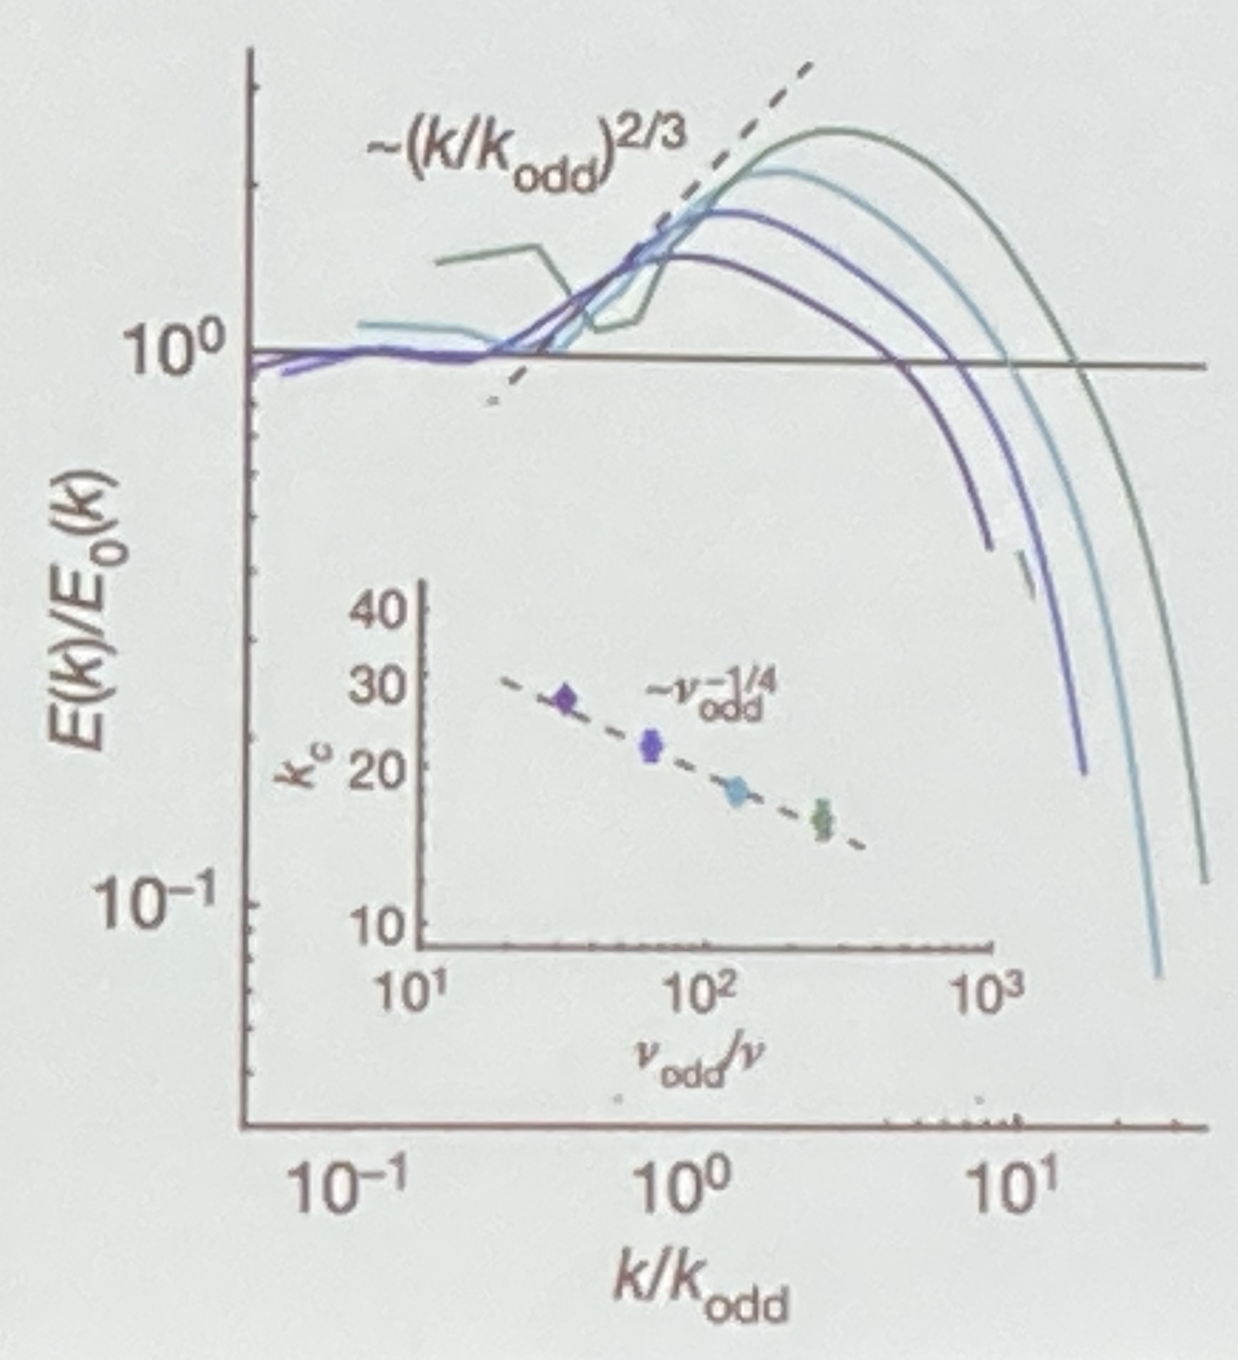
\includegraphics[scale=0.3]{Lectures/Images/lec16-nuscaling.png}
\end{center}

The theory underlying this is that we have pattern formation from two energy fluxes meeting at a particular characteristic lengthscale. Another takeaway - we have a system that behaves as 3D in low $k$, behaves as 2D in high $k$ (and displays a mixed cascade) and the interplay gives rise to some interesting phenomenology. Thus concludes our discussion of turbulence!

This lecture covers what you need for problem 1 of the homework. On Monday we do a problem solving session for problem 2. In the last lecture, we study pattern formation and phase transitions, giving you the tools for problem 3.